% interactapasample.tex
% v1.05 - August 2017

\documentclass[]{interact}

%\usepackage{epstopdf}% To incorporate .eps illustrations using PDFLaTeX, etc.
%\usepackage[caption=false]{subfig}% Support for small, `sub' figures and tables
%\usepackage[nolists,tablesfirst]{endfloat}% To `separate' figures and tables from text if required
%\usepackage[doublespacing]{setspace}% To produce a `double spaced' document if required
%\setlength\parindent{24pt}% To increase paragraph indentation when line spacing is doubled

%\usepackage[longnamesfirst,sort]{natbib}% Citation support using natbib.sty
%\bibpunct[, ]{(}{)}{;}{a}{,}{,}% Citation support using natbib.sty
%\renewcommand\bibfont{\fontsize{10}{12}\selectfont}% To set the list of references in 10 point font using natbib.sty

\usepackage[natbibapa,nodoi]{apacite}
\setlength\bibhang{12pt}
\renewcommand\bibliographytypesize{\fontsize{10}{12}\selectfont} 

%\usepackage[natbibapa,nodoi]{apacite}% Citation support using apacite.sty. Commands using natbib.sty MUST be deactivated first!
%\setlength\bibhang{12pt}% To set the indentation in the list of references using apacite.sty. Commands using natbib.sty MUST be deactivated first!
%\renewcommand\bibliographytypesize{\fontsize{10}{12}\selectfont}% To set the list of references in 10 point font using apacite.sty. Commands using natbib.sty MUST be deactivated first!

\theoremstyle{plain}% Theorem-like structures provided by amsthm.sty
\newtheorem{theorem}{Theorem}[section]
\newtheorem{lemma}[theorem]{Lemma}
\newtheorem{corollary}[theorem]{Corollary}
\newtheorem{proposition}[theorem]{Proposition}

\theoremstyle{definition}
\newtheorem{definition}[theorem]{Definition}
\newtheorem{example}[theorem]{Example}

\theoremstyle{remark}
\newtheorem{remark}{Remark}
\newtheorem{notation}{Notation}

\begin{document}

\articletype{Research Article}% Specify the article type or omit as appropriate

\title{Team Contingent or Sport Native? A Bayesian Analysis of Home Field Advantage in Professional Soccer}


%\author{
%	\name{C. J. Duan\textsuperscript{a}\thanks{CONTACT C. J. Duan, Email: %research@dulun.com} and Ananyo Chakravarty\textsuperscript{b}}
%	\affil{\textsuperscript{a}Northern Arizona University, Flagstaff, AZ 86011-5066, %U.S.A.; \textsuperscript{b}Sorrell College of Business, Troy University, Troy, AL %36082, U.S.A.}
%}


\maketitle

\begin{abstract}
%Home Field Advantage (HFA) was traditionally defined in terms of the winning percentage of home games at the team level. 
We elevate the popular Log-Normal model of Home Field Advantage from the game level to season, and sport(professional soccer) levels. Using scoring performance data from ESPN FC, we fit a Bayesian multilevel nested model to the parameters in our proposed hierarchical model of HFA, allowing information obtained from the season level to inform the inferences about scoring capabilities at the upper team and sport levels. On the one hand, our analysis reveals that much of HFA is attributed to the nature of the sport of interest. Team level sources of HFA , on the other hand, can only be attributed to a handful of clubs among 98 studied. 
%While only a handful of teams out of 98 in top 5 European leagues enjoy statistically significant HFA, we found absolutely no teams suffer from home disadvantage. Finally in the model-checking step of Bayesian analysis, we conduct comparative evaluation of the predictive accuracy of our three-level hierarchical model to that of a collapsed model with just one estimand for all team-seasons. 
%The results seem to endorse the view that home filed advantage is mainly characteristic of the sport rather than participating teams, with few exceptions.   
\end{abstract}
\begin{abbreviations}
	\textbf{HFA}-Home Field Advantage; \textbf{HWP}-Home Winning Percentage; 
\textbf{AWP}-Away Winning Percentage; \textbf{UEFA}-Union of European Football Associations; \textbf{MHG}-Most Home Goals; \textbf{MAG}-Most Away Goals
\textbf{CI}: credible interval; \textbf{IFAB}-International Football Association Board; \textbf{VAR}-video assistant referee 
\end{abbreviations}  
\begin{keywords}
	European professional soccer leagues; Home Field Advantage; Poisson generative process; Stan and CRAN-R; Predictive accuracy and Credible Intervals (CI)
\end{keywords}


\section{Introduction}

In professional team sports, the term home field advantage (HFA) – also called home advantage, home ground or home court advantage, defender's advantage, home-ice advantage – describes the benefit that the home team is believed to gain over the visiting opponent. Its scientific definition is "the consistent finding that home teams in sport competition win over 50\% of the games played under a balanced home and away schedule" \cite[p. 13]{Courneya1992}.
Due to the existence of HFA, many vital games, such as playoff or elimination matches, in major professional sports have special rules for determining which match is played at which place. The combined revenue of the Big Five European soccer leagues (English Premier League, Spanish La Liga, French Ligue 1, Bundesliga, Italian Serie A) more than doubled to 15 billion euros in 10 years from 2006/07 to 2016/17. The financial implications might partially explain UEFA's (the Union of European Football Associations) decision that a second leg of any Champions League knock-off series is favorable to playing away with the the scores still in balance after the first leg competition \citep{atkins2013}.


%[insert Figure 1 here]\\

%----------------------
%\begin{figure}[ht]

%	\centering\includegraphics[width=0.8\textwidth]{HFA_Figure_1.pdf}.
%	\caption{\textit{Revenue of the top European soccer leagues (Big Five*)	
 %from 2006/07 to 2016/17 (in billion euros)}}					 
%	\label{fig11}
%\end{figure}
%------------------------ 

The existence of HWP (home winning percentage) -denominated HFA measure has been well documented for a variety of sports, even though the contributing factors are still being debated. In their book \textit{Scorecasting}, \cite{moskowitz2012scorecasting} compiled the HWPs in all the major sports with some datasets going back as further as 1903 for MLB and 1966 for NFL. MLS figures date back to only 2002, but show the strongest evidence of HWP of 69.1\%. MLB figures, on the other hand, yield the lowest HWP of only 53.9\%. This disparity raises an important high-profile question: ``Are all sports created equal in terms of HFA?''. A subsequent but related question is ``Is HFA primarily determined by the sport being played or teams who play the sport?''. Answering such questions demands a completely new way of conceptualizing HFA and signals a major departure from the reigning framework proposed by \cite{Courneya1992}, which hinges on game being the unit of analysis.  

A second motivator for this study is related to the treatment of sports data in general, and scoring in soccer matches in particular. HWP based measures tend to upstage and upgrade the originally discrete count-based outcome to continuous type, while ignoring the underlying data generating process. To complicate matters further, consider the two extreme cases of all winning and losing regular season. The HWP and AWP(away winning percentage) are equal, taking values of either 1.o or 0.0. If we adopt HWP as the sole indicator of HFA, we go straightforward to absurd conclusions - the all winning club enjoys 100\% HFA and the zero-win team suffers from 100\% home field disadvantage.   

The current conceptualization and operationalization of HFA prompt us to take an alternative route in search of the true latent HFA underlying the numbers in record books. Specifically, we seek in this paper to achieve the following goals: 

\begin{enumerate}
	\item  Propose a fresh new vertical hierarchical model of HFA, complementing the existing horizontal framework.
	\item Highlight the different generative process underlying most sports performance metrics and suggest corresponding approaches for analysis.
	\item Sort sources of HFA simultaneously into respective sport, team related contributions.
	\item Foster a refreshing perspective on exposition of HFA and advocate exploring inter-sport HFA as a potential venue for future research.
\end{enumerate}

The remainder of the paper is structured as follows: In the section immediately after this opening introduction, we review relevant literature and assemble existing knowledge for the development of our unique hierarchical view of HFA. 
In the section of \textit{Definition of the Hierarchical Model}, we construct a full HFA-specific probabilistic model, which is mainly a joint probability distribution for all observed and latent quantities in a problem, consistent with domain knowledge and the data collection process.
In the next section of \textit{Data and Results}, we compute and display the posterior distributions of the unobserved model parameters, given the observed data collected from ESPN FC website. Also in the same section, we evaluate the fit of the hierarchical model in the context of model comparison and posterior predictive checking. We close our paper with limitations and directions for future HFA research.

\section{Review of Literature} 

%The UEFA oversees 55 European country-level member associations (such as the English Football Association- EFA), which in turn oversees all professional football leagues within their respective jurisdictions. Figure 2 provides a rough sketch of the organizational structure of professional football in Europe, with an emphasis on the elite Top 5. According to UEFA's mission statement,``UEFA's core mission is to promote, protect and develop European football at every level of the game, to promote the principles of unity and solidarity, and to deal with all questions relating to European football ... UEFA is an association of associations based on representative democracy, and is the governing body of European football. Football is the priority in everything that we do''. In conjunction with its 55 member associations, the union strives to nurture and promote the European refereeing sector  and ensure that newcomers to the UEFA list are given the proper training for their duties.

The speed and movement in top-level football competition, allied to the intense scrutiny of media on the actions on the field, means that officiating crews must be well-prepared, possess the tactical acumen, the mental strength to withstand pressure and the ability to take split-second decisions with confidence and consistency. Such split-second decisions made under severe pressure from home crowds have been proved to show systematic favoritism for the home squad   
both experimentally \citep{Nevill1999, Nevill2002} and in observational settings \citep{Nevill1996, DOHMEN2008}.

%[insert Figure 2 here]\\
%------------------------------------------------
%\begin{figure}
%	{\includegraphics[width=1.0\linewidth]{HFA_Figure_2_1.pdf}}
%	\label{fig21}
%	\caption{The Hierarchical Structure of Professional Soccer }		
%\end{figure} 
%------------------------------------------------ 

Following the episode of hooligan-induced riot on Feb. 2, 2007, the Italian authorities forced soccer clubs with deficient security standards at their home stadiums to play their home games with no spectators. The ruling inadvertently created a sizable and scarece sample of 21 professional soccer games played before empty bleachers. \cite{Pettersson-Lidbom2010} seized on this historical opportunity and contrasted the performance metrics of both referees and players by looking at the matches played by the same team and officiated by the same referee crew. They found convincing evidence for the effect of spectators on referees, manifested in the 70\% (26\%) drop for red (yellow) cards issued favoring the home team. On the other hand, the players did not seem to play any differently whether the yelling crowds were present or absent. 

With game as the anchoring unit of analysis, \cite{Courneya1992} developed a conceptual framework along the timeline axis of a typical soccer game. For simplicity of reference and purpose of contrasting, we designate their framework as the horizontal view of HFA (HVHFA). From left to right along the axis, HVHFA incorporates five major components: game site location, game location factors, psychological states, behavioral sates, and the final performance outcomes. At the end of their review, they pointed out that future research should be directed at factors causing HFA rather than the verification of its existence. After taking stock of decades' HFA research findings suffused with equivocality, \cite{Carron2005} surprisingly revised the original HVHFA with the deletion of ``officials'' and the inclusion of ``psychological states''. The rationale behind their removal of officiating factors is rather methodological inconvenience. Unlike spectators, players and coaches, referees and umpires can't be easily assigned to either hosting or visiting status for each game they officiated. 


\cite{Pollard1986} discovered that the extent of HFA in English soccer has remained relatively consistent since the formation of the English Football League in 1888. The time-invariant tendency, coupled with the largest betrayed effect, makes professional soccer an excellent venue for studying HFA at a more aggregate level beyond individual matches and even seasons. 

As \cite{Boyko2007} pointed out, traditional frequentist statistical approaches don't address whether referees or players alone or combined channel crowd effects to impart on final match outcome. Bayesian inferential approach separates itself from its frequentist counterpart due to its emphasis on modeling all forms of uncertainty rather than providing point estimates. Regardless of the inferential approaches taken, one major goal of statistical analysis is model selection among a set of competing models that were assumed to have generated the observed data. With the aid of posterior predictive checking \citep{Gelman1996}, researchers can assess the fitness of competing models with realized discrepancies between the actual and replicated data points. 

With the rare exceptions of \cite{doi:10.1080/02664760802684177}, \cite{Gajewski2006} and \cite{Glickman1998, Glickman2005}, Bayesian statistical approach has not been widely adopted in the analysis of HFA. One unique feature of the \cite{Gajewski2006} study is that they model longitudinal data across seasons while utilizing a unique HFA parameter dedicated to each team involved in the investigation. One problem common to these Bayesian studies is that they directly model the match-based goal differentials between the hosting and visiting teams. Although Poisson-logNormal models \citep{doi:10.1080/02664760802684177,doi:10.1111/1467-9884.00366} treat host goals and visitor goals separately, model parameters such as home advantage, offensive and defensive scoring intensities still were estimated simultaneously using game-level observed pairs of goals.   Such estimates based on score differentials  or score-pairs of individual matches are effectually  blending home team's HFA and visitors' guest field disadvantage. Thus, we sense an urgent need to break down HFA into sub-components, which we can pinpoint to their originating sources.    

The subject and methodology-matter motivations for this research lie in the decomposition of home field advantage in a multilevel format that naturally reflects the structure of professional soccer competition. With the help of Bayesian nested modeling, we shall demonstrate next how easily we can alter the structural complexity of the main candidate model with just a few lines of code.

%[insert Figure 3 here]\\
%------------------------------------------------
%\begin{figure}[h]

%	{\includegraphics[width=1.0\linewidth]{HFA_Figure_3_1.PNG}}
	
%	\caption{The Hierarchical Model of Home Field Advantage }	
%	\label{fig33}
%\end{figure} 
%------------------------------------------------ 

\section{Definition of the Hierarchical Model} 

The essence of Bayesian inference is fitting a probability model to a dataset and generating probability distributions on the parameters encapsulated by the model \citep{Gelman2014}.





For our project, the data set contains the season-level best home and away scoring numbers ($y^H_{is}$ and   $y^A_{is}$ respectively) of each club i in the Top 5 leagues. 
%As shown in figure \ref{fig33}, our hierarchical model reflects the organizational structure of professional soccer shown in figure \ref{fig21}. 
We treat the generative processes of $y^H_{is}$ and $y^A_{is}$ as similar but independently governed by their own respective parameters. At the measurement level, we encode $y^H_{is}$ and $y^A_{is}$ into corresponding latent scoring rate $\lambda^H_{i}$ and $\lambda^A_{i}$ with Poisson distribution, which is a commonly accepted distributional model for sports count data \citep{Miller2015}:

 Instead of modeling directly HFA as constant for all teams across seasons,we acquire inference about the team level HFAs ($\delta_i$) by assessing the difference between the latent scoring intensity $\theta^H_{i}$ and $\theta^A_i$. By the same token, we can derive sport-level HFA ($\Delta$) via assessing the differential between the hyperparameters  $\mu^H$ and $\mu^A$. We specify the hierarchical model of HFA formally as a set of equations consisting of (\ref{eq1}), (\ref{eq2}), (\ref{eq3}). 

\begin{equation}
\begin{cases}
y^H_{is} \sim \text{Poisson}(\lambda^H_{i})\\
y^A_{is} \sim \text{Poisson}(\lambda^A_{i})
\end{cases}
\label{eq1}
\end{equation}



\begin{equation}
\begin{cases}
\log\lambda^H_{i} = \theta^H_{i}\\  
\log\lambda^A_{i} = \theta^A_{i}\\
\delta_i = \theta^H_i - \theta^A_i
\end{cases}
\label{eq2}
\end{equation} 

\begin{equation}
\begin{cases}
\theta^H_i \sim Normal(\mu^H, \tau^H)\\
\theta^A_i \sim Normal(\mu^A, \tau^A)\\
\Delta = \mu^H - \mu^A
\end{cases}
\label{eq3}
\end{equation} 

%As outlined in above equations, the total number of parameters included in the full model is 208, including two $\mu$ and two $\tau$ at the top + 2 X 98 team-level $\delta$. In addition, there are two hyper-parameters ($\sigma$) governing the distribution of league and team level parameters. 

%In addition to our main multilevel model outlined above, we also fit an alternative one-level-fits-all model with only one estimand for all teams in every league. Its mathematical form is given in equation 4 and 5, with the disappearance of i and j on the right hand side. Equation \ref{eq5} and \ref{eq6} represent our (prior to seeing data) belief that there is no such thing as HFA.

%\begin{equation}
%\begin{cases}
%y^H_{is} \sim \text{Poisson}(\lambda^H)\\
%y^A_{is} \sim \text{Poisson}(\lambda^A)
%\end{cases}
%\label{eq5}
%\end{equation}

%\begin{equation}
%\begin{cases}
%\Delta = \lambda^H - \lambda^A\\
%\lambda^H, \lambda^A \sim cauchy(0, 10)
%\end{cases}
%\label{eq6}
%\end{equation} 

\section{Data and Results} 

For practical reasons, the Top 5 leagues serve as a convenient sample as performance data at season level are reliable and retrievable via internet.  On ESPN FC website, we find a pair of venue-delineating (home and away) goal scoring metrics used to characterize a professional soccer club's regular season. Below, we define those statistics using the 2015/16 La Liga season of Real Madrid C.F. as an example.

\begin{itemize}
	\item Most Home Goals (as $y^H_{is}$) = maximum goals scored in a single match played at home. For the season 2015/2016, Real Madrid’s $y^H_{3,1,16}$ is 10. They beat Rayo Vallecano by 10-2 at Santiago Bernabéu Stadium on 12/20/2015.
	\item Most Away Goals (as $y^A_{is}$) = maximum goals scored in a single away match. For the season 2015/2016, Real Madrid’s $y^A_{3,1,16}$ is 6. They defeated Espanyol 6-0 on 9/12/2015 at RCDE stadium.
\end{itemize}

Table 1 provides the summary statistics of $y^H_{is}$ and $y^A_{is}$. Both averages and medians evince the existence of positive goal differential between maximum home and away goals. However, the MAG is more skewed than MHG in that the max. of MAG is actually greater than that of MHG. Deletion of such outliers is not an option in conducting sports analytics, because they are quintessential of the underlying exceptional performance by athletes. Fortunately, Bayesian statistics can accommodate such wide dispersion of data points with alternative distribution functions other than the commonly-applied Gaussian PDF (normal probability density function). 

%------------------------------
%[insert Table 1 here]\\
%-----------------------
\begin{table}[h]
	\tbl{Descriptive Statistics}
	{\begin{tabular}{cccccccc}\toprule
		
		& Mean & Median & Std. Dev. & Min. & Max. & Skewness & Kurtosis\\ \midrule
		MHG ($y^H_{js}$) & 3.634 & 4 & 1.676 & 0 & 9 & 0.246 & 0.034 \\
		
		MAG ($y^A_{is}$) & 2.884 & 3 & 1.676 & 0 & 10 & 0.627 & 0.786 \\ \bottomrule
		
	\end{tabular}}
	\label{tab1}
	\tabnote{Goal Scoring Metrics: Most Home \& Away Goals at the Season Level} 
\end{table}
%=====================================================

We fit our model with 4 chains of length 999 (with the first 1/3 for warmup) using the default sampler in Stan, the HMC variant of No-U-Turn Sampler (NUTS) \citep{Hoffman2014}.  

%[insert Figure 4 here]\\

\begin{figure}
	{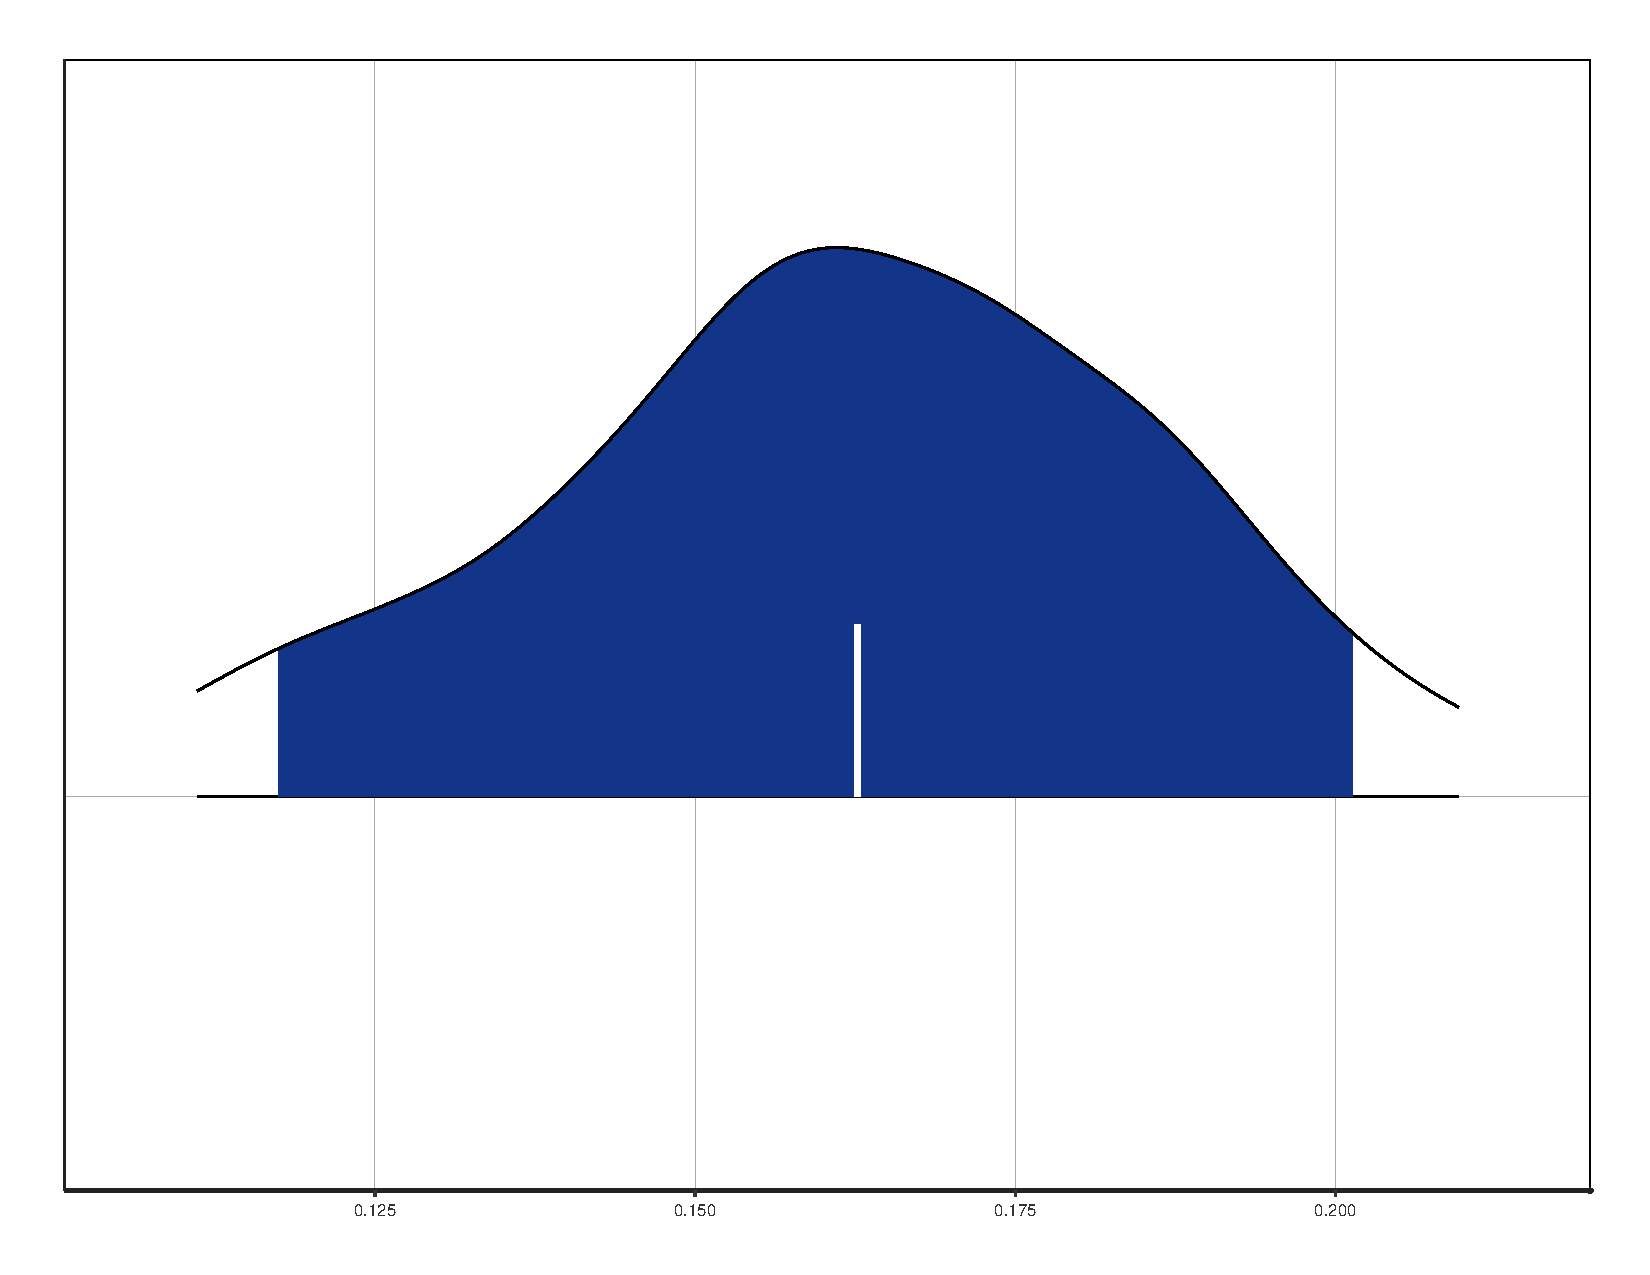
\includegraphics[width=0.9\linewidth]{HFA_Posterior_Sport.pdf}}
	\caption{Posterior Density Plot ($\Delta$) HFA Impact at Sport Level}	
	\label{fig1}
\end{figure}


The sport level estimates of goal-scoring rate differential are shown in figure \ref{fig1} as shift from the 0. The outer contour line depicts the 95\% uncertainty intervals, while the shaded area underneath covers the corresponding 90\% uncertainty intervals. The light bar in the middle represents the mean. From figure \ref{fig1}, we observe absolutely strong (95\%) manifestation of HFA for the sport of soccer (in the top panel). The goal-scoring differentials are centered around 0.16 goals with comparable lengths of uncertainty intervals. 
%In the bottom panel of figure \ref{fig4}, we see no signs of HFA and the Top 5 leagues as a whole did not assert much influence on either location or shape of the parameters of interest. The English Premier League was the only league  able to slightly push the center to the right of 0.0-dotted line.


 
To summarize team level estimates, we use the inner thick line to represent the 90\% uncertainty interval and the outer thin line for 95\% uncertainty level respectively. The dot in the middle still represents the mean as before. As shown in figure \ref{fig2}, Real Madrid is the only club among all 20 in La Liga enjoys strong HFA with 95\% CI (credible Interval). Another five clubs exhibit only moderate HFA with 90\% CI not encompassing the null 0 point.  

\begin{figure}
	{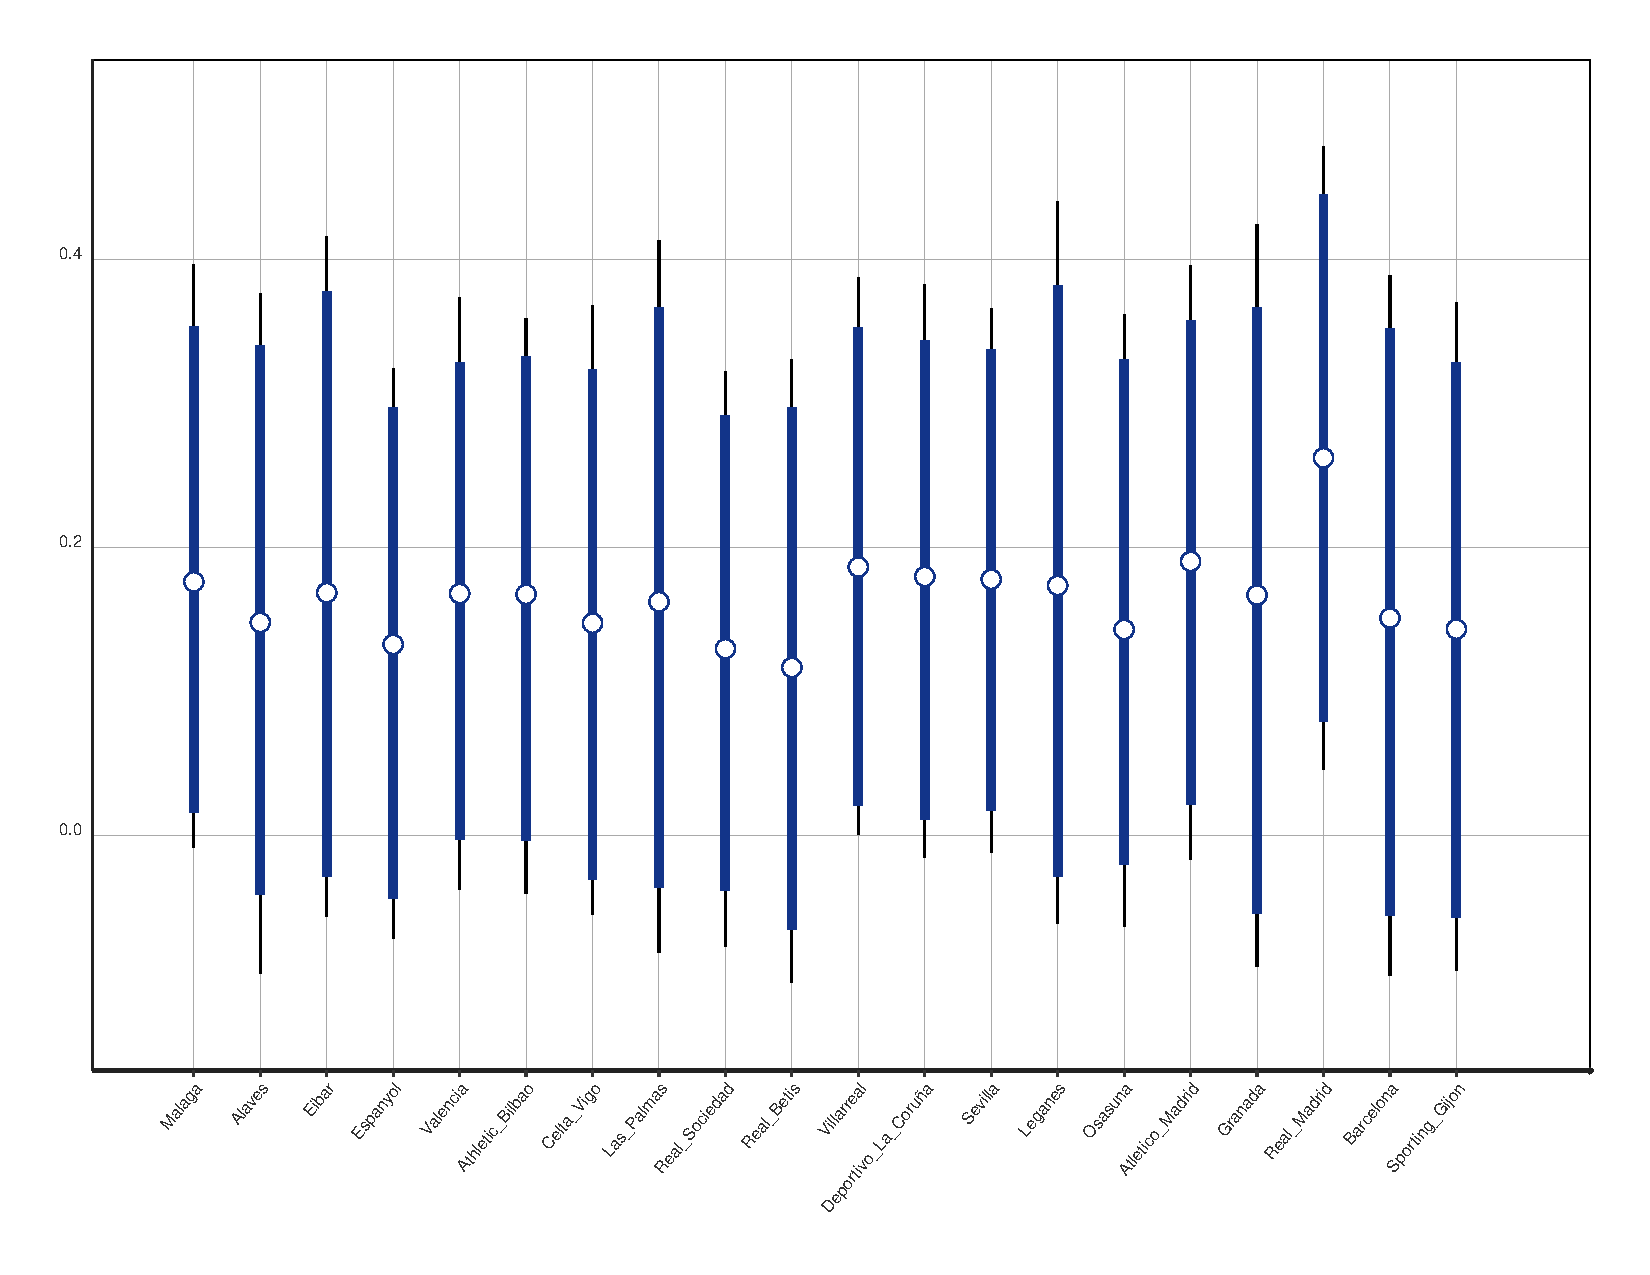
\includegraphics[width=0.9\linewidth]{HFA_Posterior_La_Liga.pdf}}
	\caption{HFA $(\delta_i)$ Posterior Plot for Clubs in La Liga}	
	\label{fig2}
\end{figure}

Among 20 teams in Serie A (shown in figure \ref{fig3}), AS Roma is the only club possess strong HFA with 95\% CI (outer thin line) not touching the null 0 line. Lazio is another team enjoys moderate HFA with 90\% statistical significance. 

\begin{figure}
	{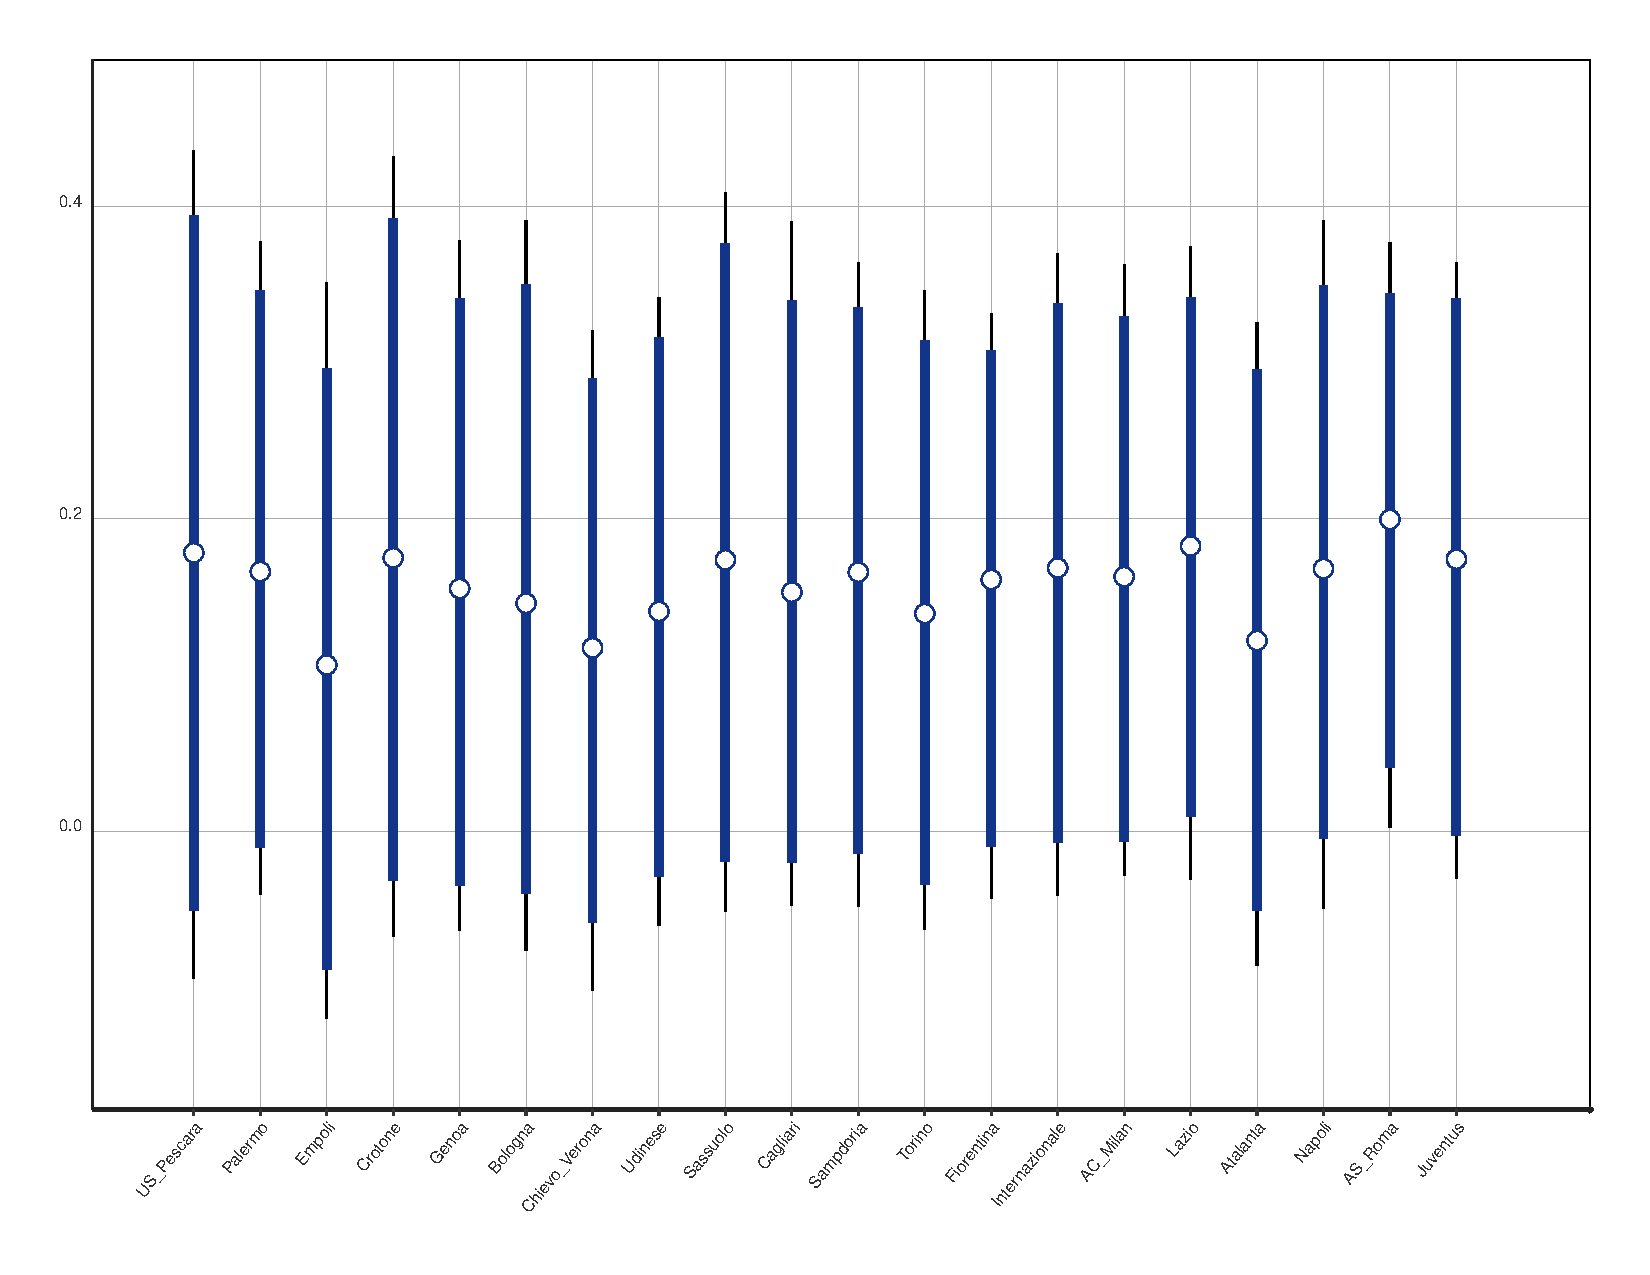
\includegraphics[width=0.9\linewidth]{HFA_Posterior_Serie_A.pdf}}
	\caption{HFA $(\delta_i)$ Posterior Plot for Clubs in Serie A}	
	\label{fig3}
\end{figure}

Among the 20 teams in French Ligue 1 (figure \ref{fig4}), PSG shows strong HFA, while Lyon and Marseilles borderline the threshold of 95\% statistical significance. Three other team enjoy HFA only to some moderate extent.

\begin{figure}
	{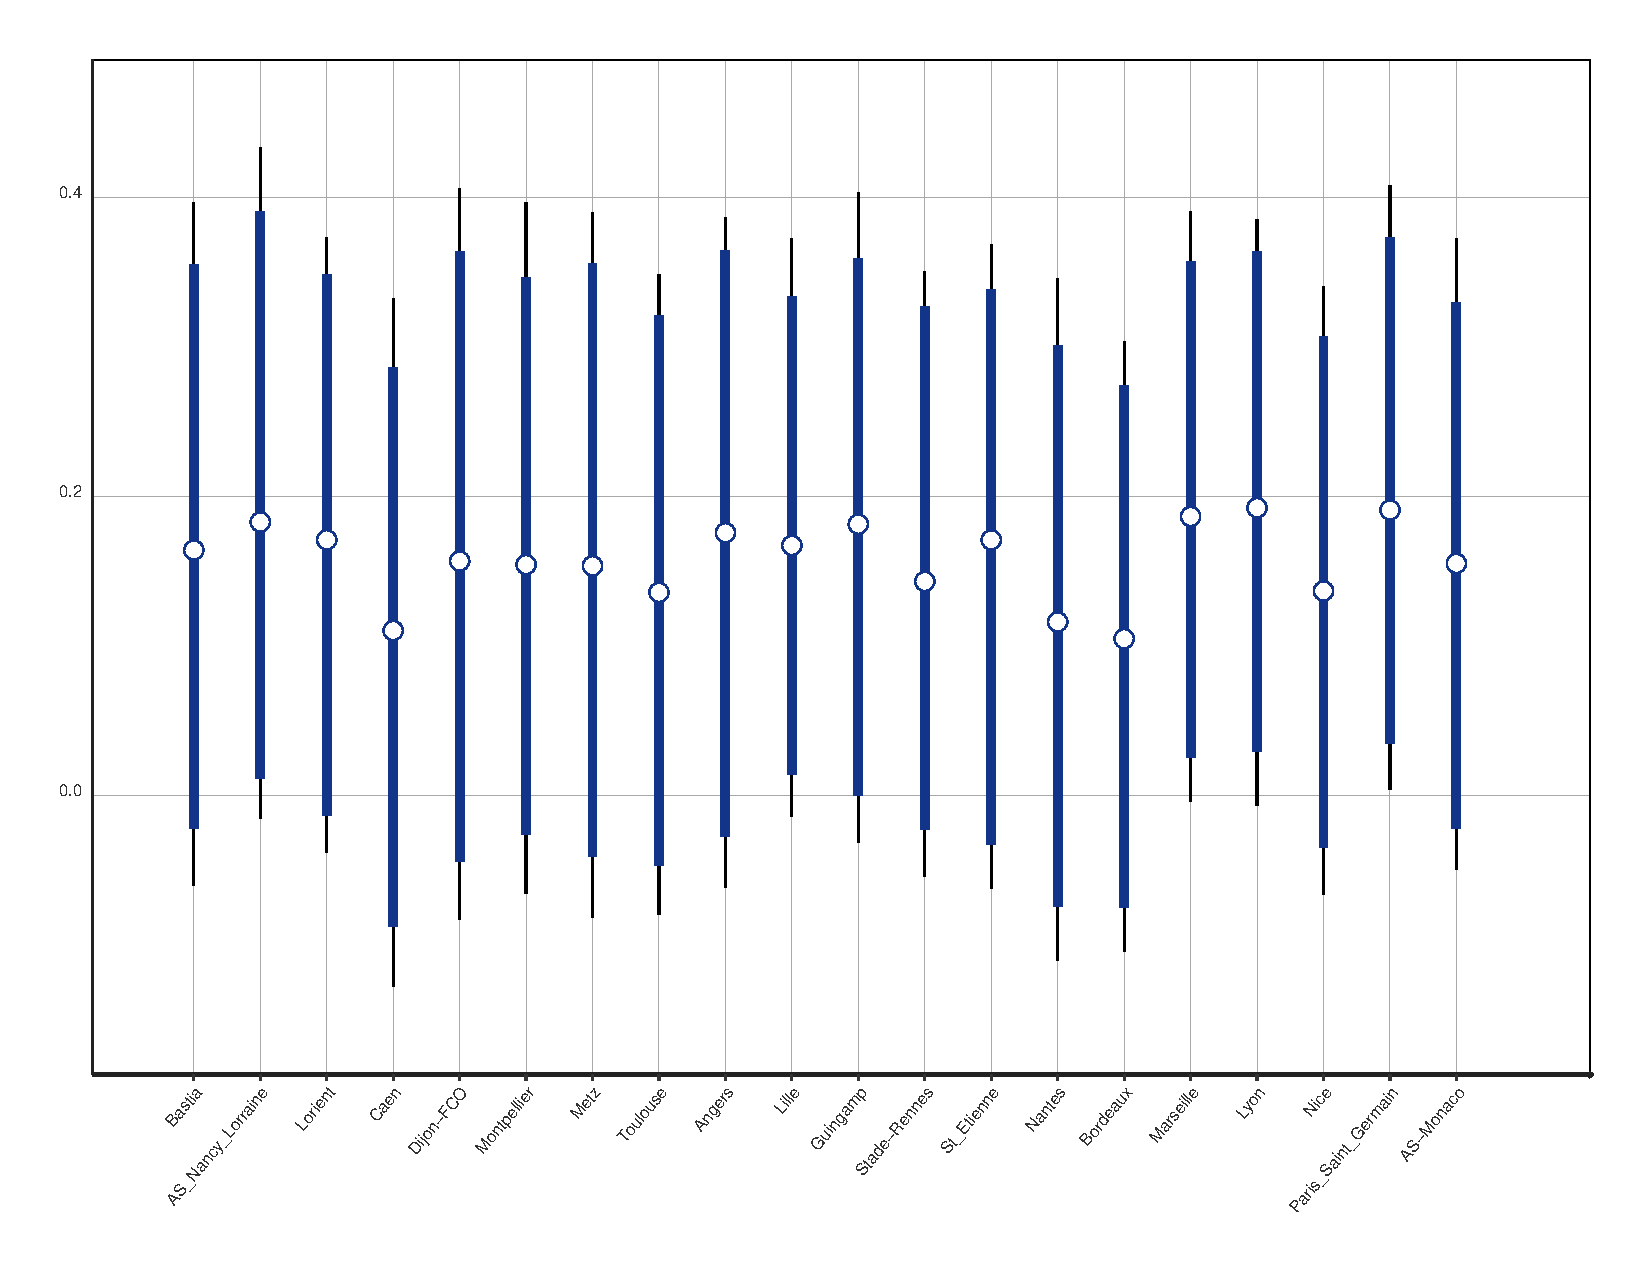
\includegraphics[width=0.9\linewidth]{HFA_Posterior_Ligue_1.pdf}}
	\caption{HFA $(\delta_i)$ Posterior Plot for Clubs in Ligue 1}	
	\label{fig4}
\end{figure}

For teams in Bundesliga as shown in figure \ref{fig5}, Bayern Munich is the one in possession of dominant HFA with 95\% statistical significance, while Hertha Berlin and Schalke 04 enjoy moderate HFA.  

\begin{figure}
	{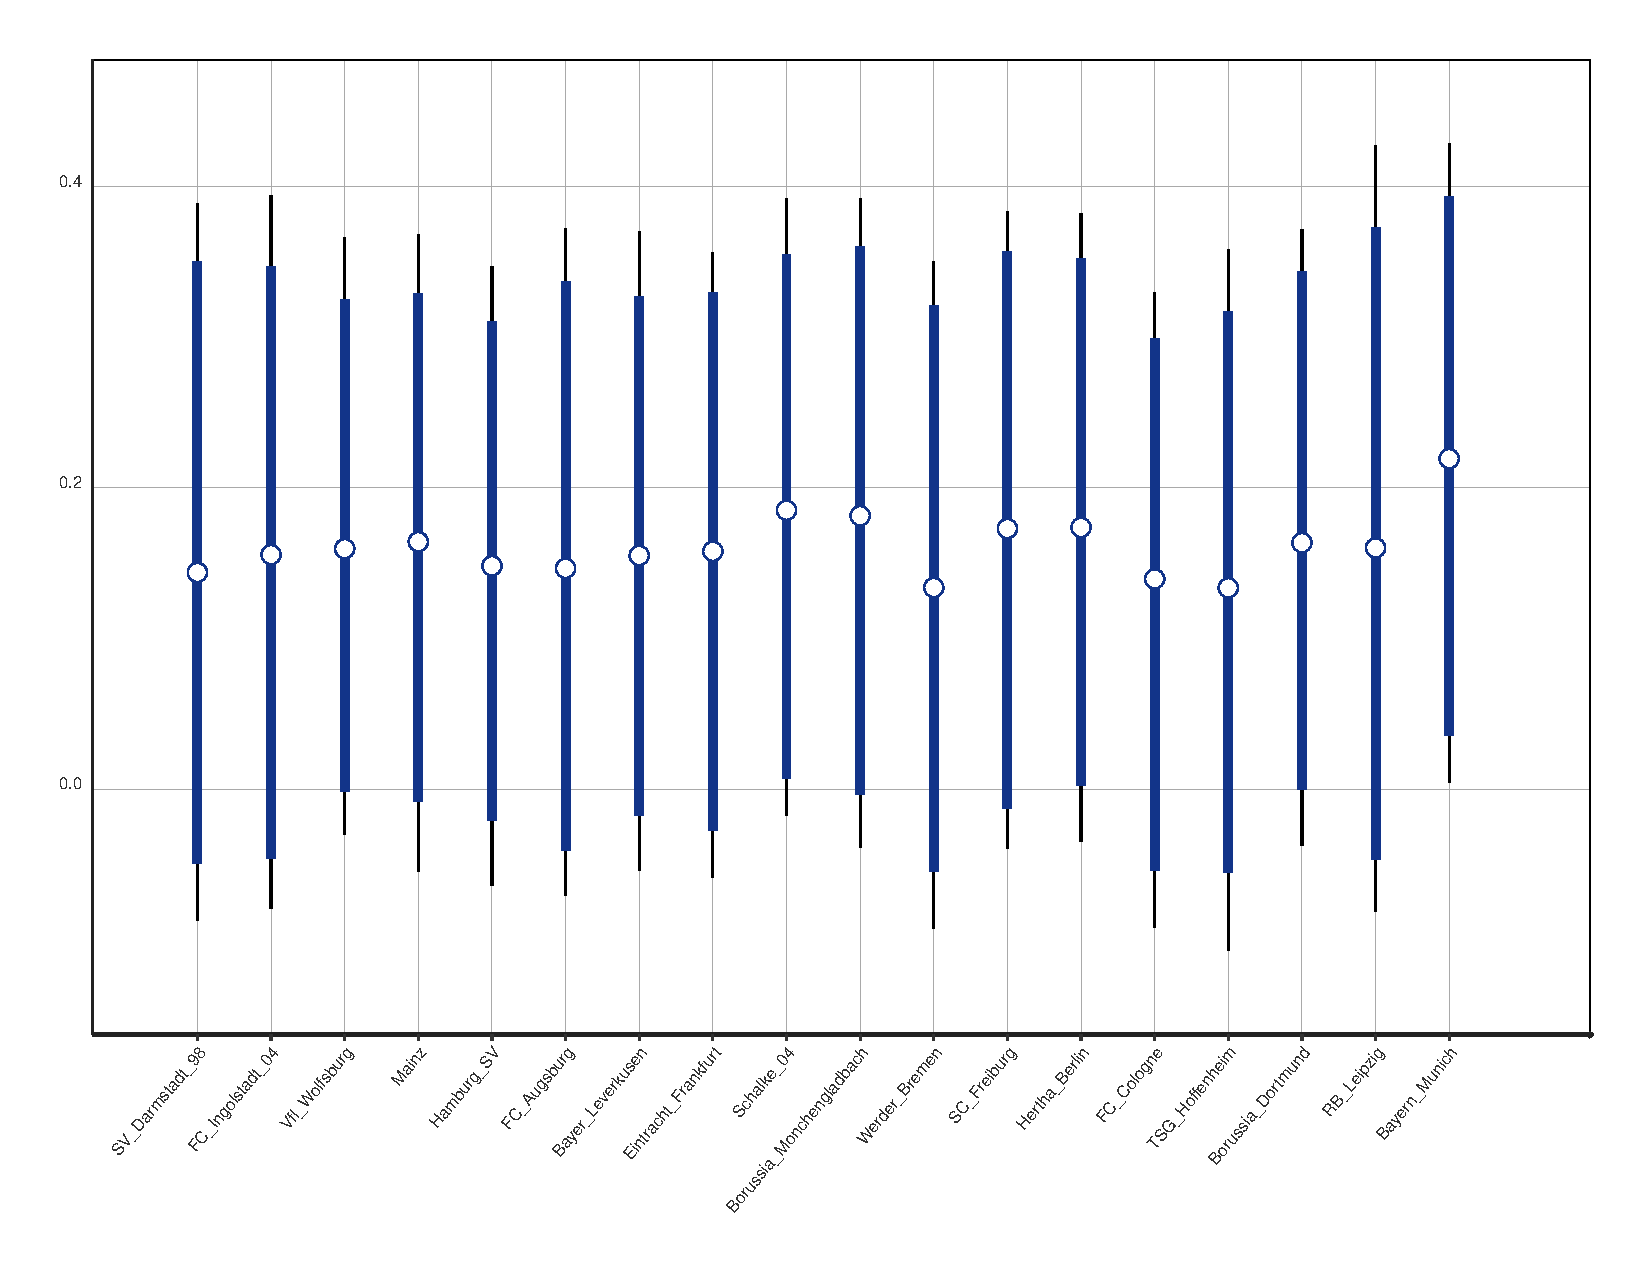
\includegraphics[width=0.9\linewidth]{HFA_Posterior_Bundesliga.pdf}}
	\caption{HFA $(\delta_i)$ Posterior Plot for Clubs in Bundesliga}	
	\label{fig5}
\end{figure}

Among teams in English Premier League (in Figure \ref{fig6}), Chelsea, Everton and Middlesbough are the three teams enjoy strong HFA, while Manchester City, Tottenham Hotspurs and Arsenal show signs of moderate HFA. 

In summary, we observe, among 98 clubs included in this study, a total of 23 teams exhibit posterior 90\% CIs not encompassing the null zero line. Further, 7 out of the 23 teams exhibit 95\% CIs not encompassing the null zero line. It is worthy pointing out that the seven clubs cherishing strong HFA include usual league champions (Real Madrid, PSG, Bayern Munich, Chelsea), as well as non-champion caliber teams like Everton and Middlesbough.  

\begin{figure}
	{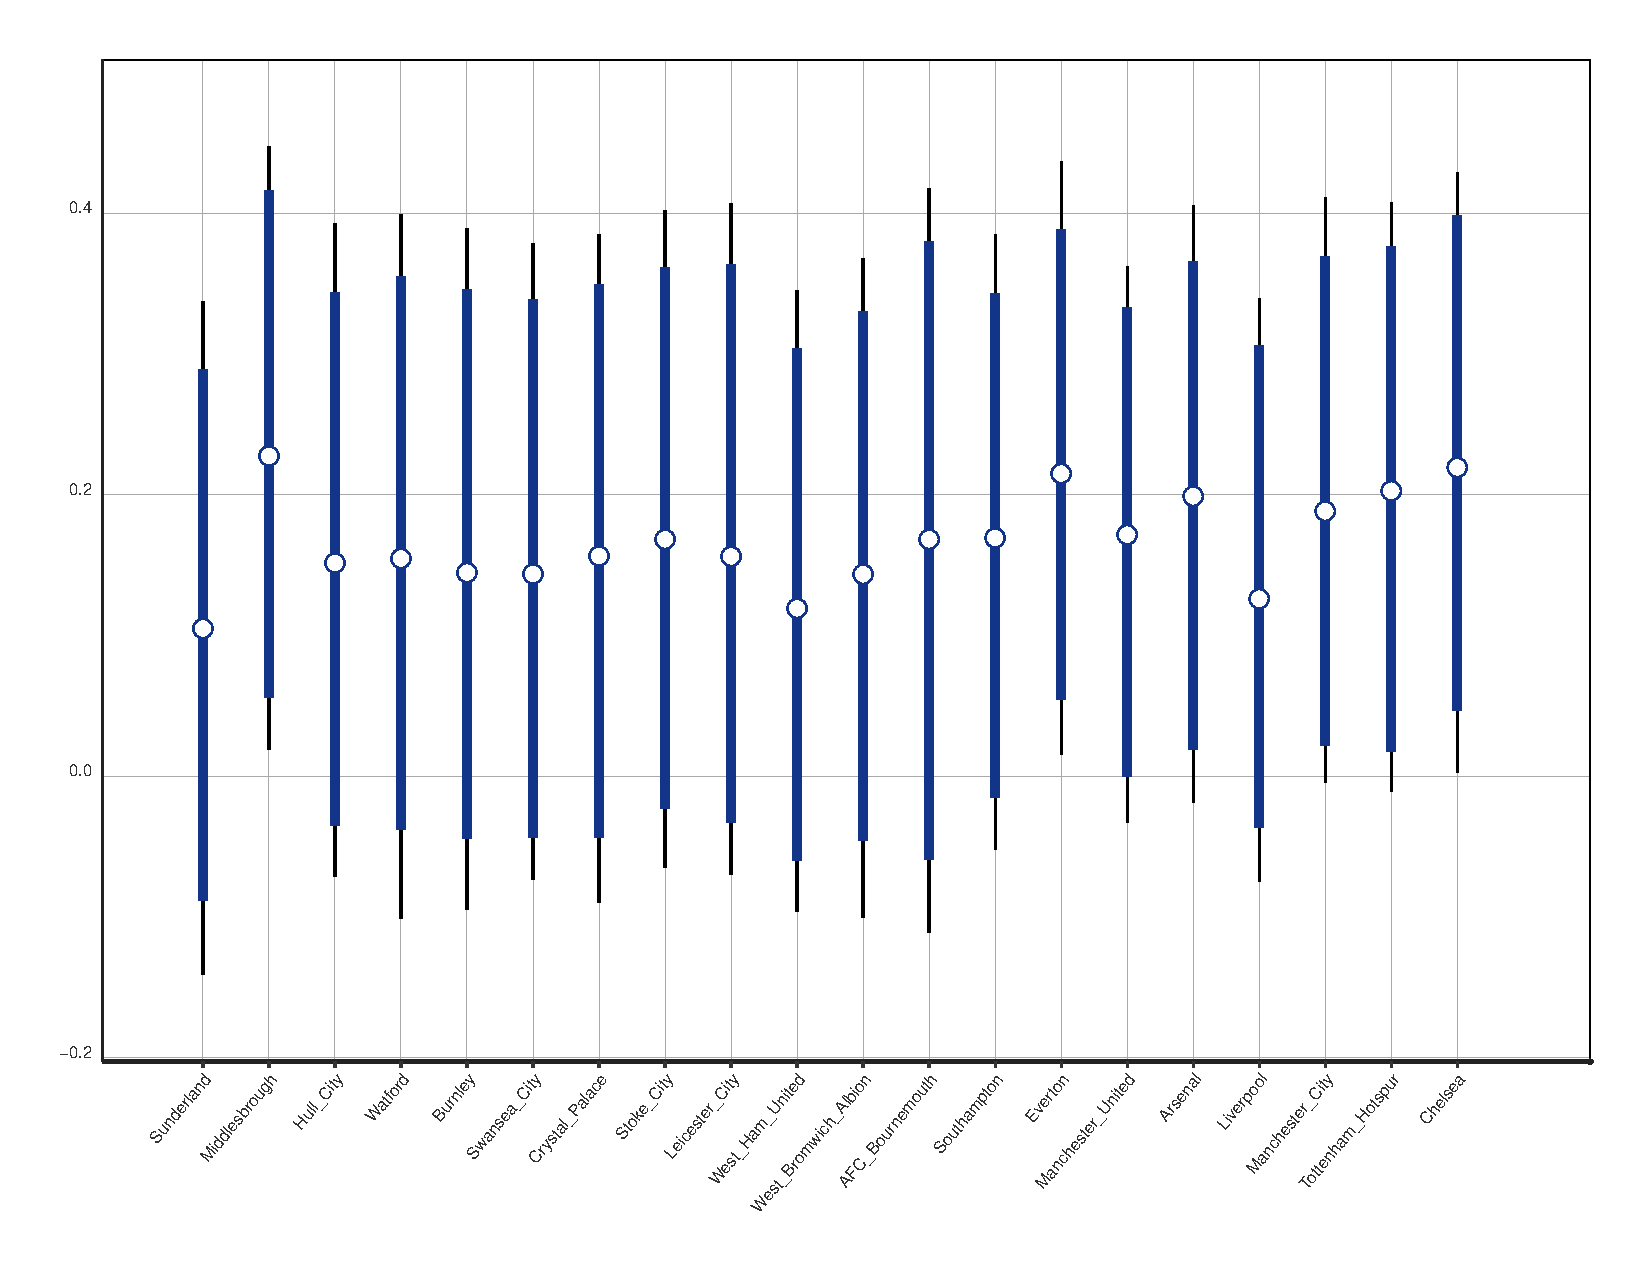
\includegraphics[width=0.9\linewidth]{HFA_Posterior_EPL.pdf}}
	\caption{HFA $(\delta_i)$ Posterior Plot for Clubs in English Premier League}	
	\label{fig6}
\end{figure}

As part of the Stan model \citep{team2015stan}, we sample replicated data for the best scoring differential - ydiff - in the \textit{generated quantities} block. We can then check whether the actual score differences are consistent with the distribution of replicated data. For each of the 1122 seasons, we compute the 50\% and 25\% uncertainty intervals (UI) based on the replicated results. We observe that all of the actual ydiffs are in the 50\% UIs and 97\% in the 25\% UIs.   

\section{Discussion}

In this work, we give home field advantage full Bayesian treatment with unique hierarchical structure. Departing from the tradition of treating HFA as a constant intercept for all teams and across seasons, we are able to model HFA indirectly and explore the locality of sources of HFA. We tested the proposed model with maximum home and away scoring data covering seasons of 2000/01 to 2016/17. The results reveal that HFA exists sport-wide while only a handful of teams command statistically significant effect. 



%Unexpectedly, we found no signs of significant HFA variation at the middle league level and lower club level. 
%A possible explanation to this finding is that the traveling distances within most European countries are within one time-zone, and therefore are unlikely to cause any anything other than negligible fatigue. This also highlights one major limitation of our study.  The inherent geographical proximity minimizes the effect of traveling induced by league-authored schedules.

%But even more remarkedly is the revelation from the post-hoc comparative analysis of goodness of fit between the single-level model and the full model. Considering the fact the single-level model already measures around 81\% in terms of predictive accuracy, we would trade off the appeal of 3\% extra improvement offered by the three-level model for the ultra-simple uni-parameter model for practical reasons. For the purpose of conducting better HFA research, we might need to reorient the research field toward a broader and more encompassing unit of analysis - sport, which dictates the rules, format, and especially on-field rulings via the referees as delegates from the governing bodies.


We all know that the home filed advantage exists in all sports with varying degrees. A great deal of future research efforts should be devoted to the inter-sport investigation of HFA and quantifying the subjectivity of refereeing standards. 
Refereeing controversies regularly arise in professional competitions. Barcelona coach Ernesto Valverde complained on March 1, 2018 about an “invisible penalty” awarded to Las Palmas during the match that ended  in 1-1 draw.
The Spanish Football Federation (RFEF) has announced it is seeking approval from the International Football Association Board (IFAB) to roll out VAR ( video assistant referee)  in La Liga at the start of the 2018-19 season. VAR is already active in the top divisions in both Italy and Germany, while in England it has been tested on a trial basis in the 2017/18 season in selected domestic cup games.

Systems like VAR in soccer are purported to correct clear and obvious refereeing errors, regarding decisions on goals, red cards, penalties and cases of mistaken identity. If implementation of such machine-assisted officiating  systems becomes widespread, we can expect a clear downward trend with regard to the effect size of home field advantage. When enough machine-generated officiating data are available, we should incorporate the technology related factors into our models accordingly and assess their contributions to our understanding of HFA at the sport level. Winning on home turf and picking up points away has long been cited as the path to success in soccer. We would argue that the same mentality is driving home field advantage, as long as the enthusiastic fans are in the stands and voicing out their enthusiasms to the right target - the referees supposedly.    
 

 


 

%\section*{Acknowledgement}

% We would like to thank ESPN FC for compiling the season-level club performance data and allow public access.


 

 
\newpage
 
\bibliographystyle{apacite}
\bibliography{Soccer, Bayesian}
 
\end{document}
